% Supercapacitor results
    \subsection{Comportement du système}

Les comportements du système ont ensuite été étudiés. Comme nous l'avons évoqué précédemment, nous souhaitons étudier la distribution des charges au sein des électrodes et les phénomènes d'adsorption des ions.

Pour ce faire, nous avons imaginé trois systèmes : un système chargé à \qty{4.0}{\volt}, un système non chargé, et un système chargé à \qty{4.0}{\volt} comportant un défaut sur une des électrodes. Le défaut choisi a été un atome de carbone manquant.\\
Pour chacun d'eux, deux simulations ont été effectuées : pour un nombre arbitraire d'ions (\num{10} paires d'ions entre les électrodes), et pour une concentration d'\qty{1}{\mole \per \liter} (soit \num{2} paires d'ions entre les électrodes).

Chacune de ces simulations a suivi le déroulement de la \autoref{sec:deroulement_simulations}, c'est-à-dire :
\begin{itemize}
    \item une minimisation à \qty{0}{\kelvin}
    \item une relaxation à \qty{300}{\kelvin} et \qty{1}{\atm} en deux étapes de \qty{0.01}{\nano \second}
    \item la simulation principale à \qty{300}{\kelvin} et \qty{1}{\atm} pour \qty{1}{\nano \second}
\end{itemize}

Les grandeurs thermodynamiques lors des différentes étapes de simulation sont présentées aux \autoref{fig:relaxation_thermo} et \ref{fig:main_thermo}. À partir de ces graphes, nous estimons que l'équilibre est atteint pour les trois systèmes à partir de \num{4000000} d'itérations soit \qty{0.4}{\nano \second} : en effet, puisque la température est contrôlée nous ne pouvons nous reposer sur sa valeur comme indication de l'équilibre ; De plus, puisque l'énergie potentielle des systèmes dépend de s'ils sont chargés ou non cette grandeur n'est pas indicative non plus ; Ainsi nous nous reposons sur la pression pour témoigner de l'équilibre du système.

\begin{figure}[h!]
    \centering
    \begin{subfigure}[t]{.49 \textwidth}
        \centering
        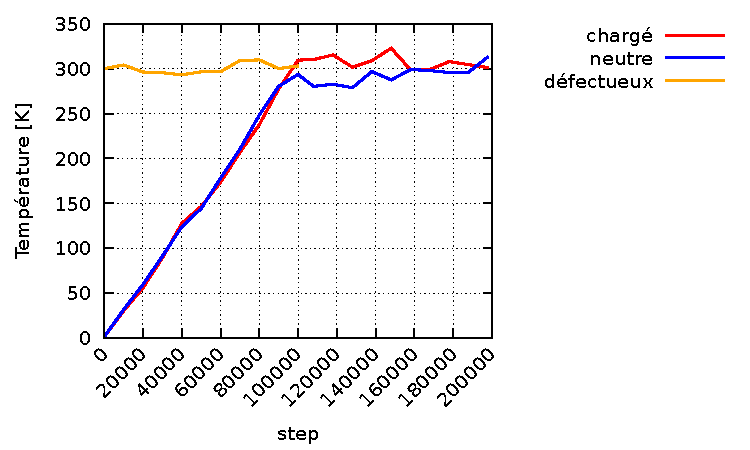
\includegraphics[width = \textwidth]{relaxation_temp.pdf}
        \caption{Température}
    \end{subfigure}%
    ~
    \begin{subfigure}[t]{.49 \textwidth}
        \centering
        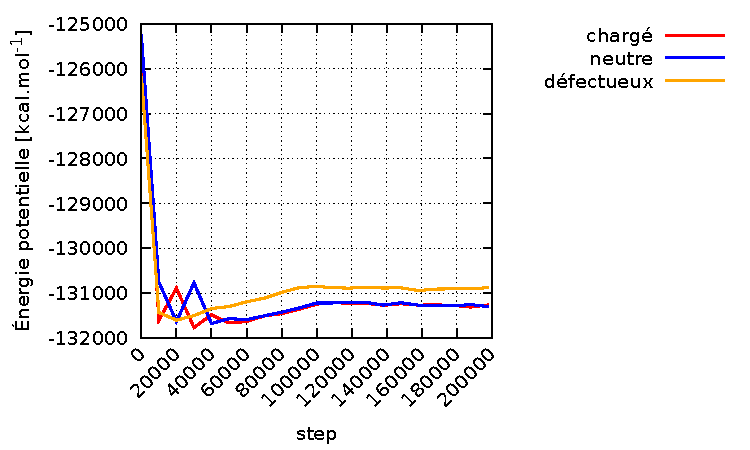
\includegraphics[width = \textwidth]{relaxation_epot.pdf}
        \caption{Énergie potentielle par atome}
    \end{subfigure}
    \begin{subfigure}[t]{.49 \textwidth}
        \centering
        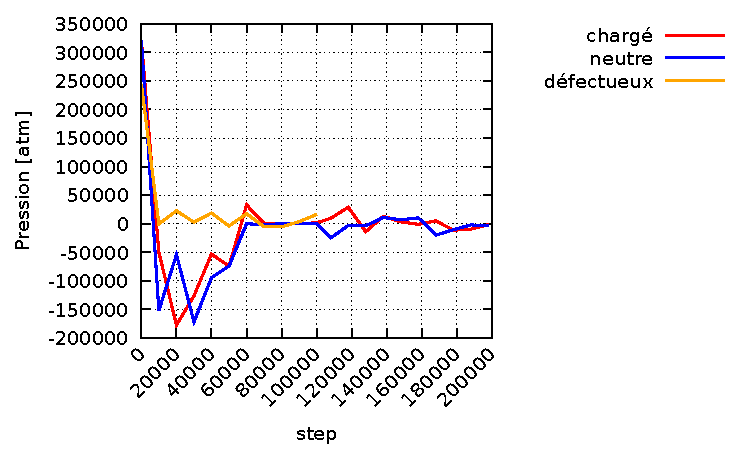
\includegraphics[width = \textwidth]{relaxation_press.pdf}
        \caption{Pression}
    \end{subfigure}
    \caption{Grandeurs thermodynamiques au cours de la relaxation et stabilisation}
    \label{fig:relaxation_thermo}
\end{figure}

\begin{figure}[h!]
    \centering
    \begin{subfigure}[t]{.49 \textwidth}
        \centering
        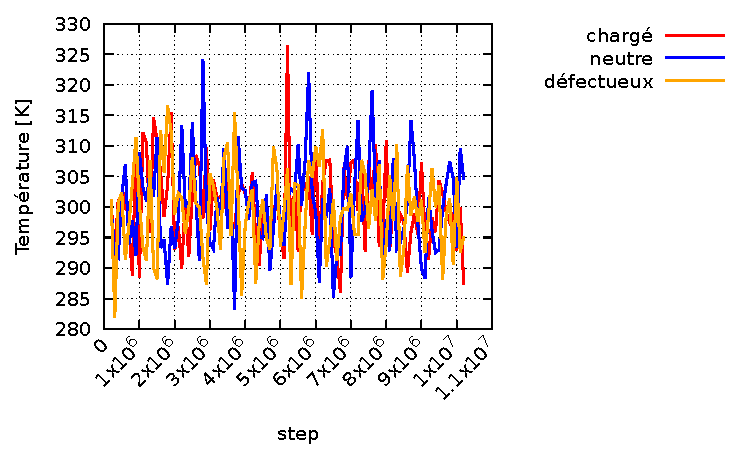
\includegraphics[width = \textwidth]{main_temp.pdf}
        \caption{Température}
    \end{subfigure}%
    ~
    \begin{subfigure}[t]{.49 \textwidth}
        \centering
        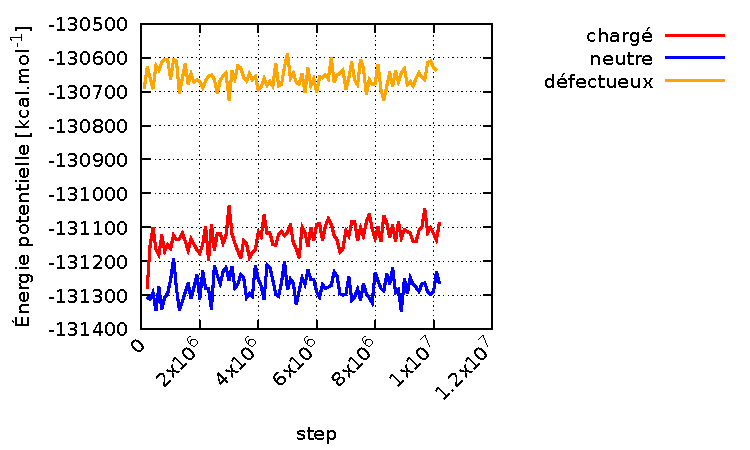
\includegraphics[width = \textwidth]{main_epot.pdf}
        \caption{Énergie potentielle par atome}
    \end{subfigure}
    \begin{subfigure}[t]{.49 \textwidth}
        \centering
        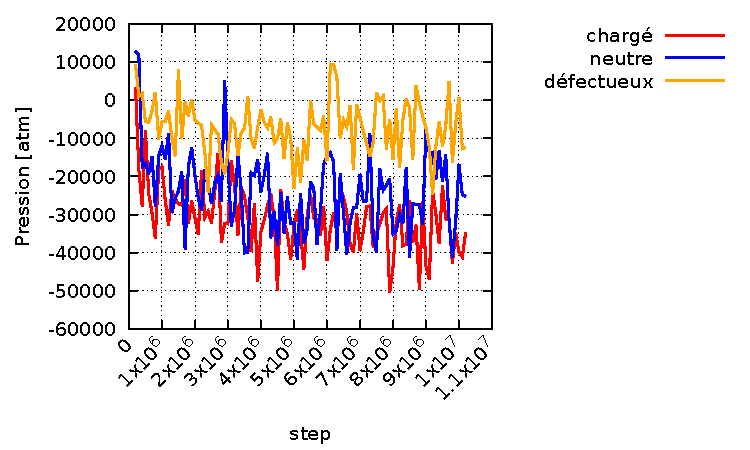
\includegraphics[width = \textwidth]{main_press.pdf}
        \caption{Pression}
    \end{subfigure}
    \caption{Grandeurs thermodynamiques au cours de la simulation principale}
    \label{fig:main_thermo}
\end{figure}

% Charge distribution on the electrode
    \subsubsection{Distribution des charges sur les électrodes}

La distribution des charges sur les électrodes est mesurée par la moyenne des charges au sein de certains groupes d'atomes. Ceux-ci sont : les atomes de carbone composant les couches extérieures des électrodes, les atomes des couches intérieures, les atomes voisins du défaut.\\
La \autoref{fig:charges_groupes} présente les différents graphes obtenus pour cette mesure pour les différents systèmes, les \autoref{fig:comparaison_ch-sc-defected} et \ref{fig:comparaison_ch-sc-neutral} présentent des comparaisons entre les systèmes, et le \autoref{tab:comparaison_charges} résume les moyennes des charges suivant le groupe d'atomes de carbone.

\begin{figure}[h!]
    \centering
    \begin{subfigure}[t]{.49 \textwidth}
        \centering
        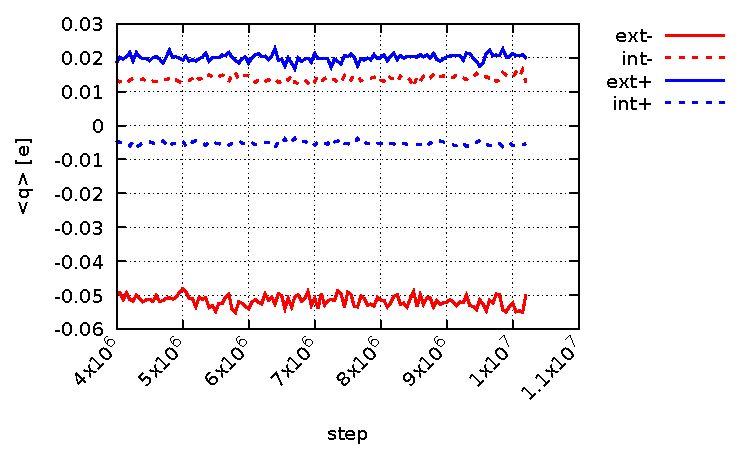
\includegraphics[width = \textwidth]{ch-sc_q-1.pdf}
        \caption{Pour le système chargé}
        \label{fig:charges_groupes_ch-sc}
    \end{subfigure}%
    ~
    \begin{subfigure}[t]{.49 \textwidth}
        \centering
        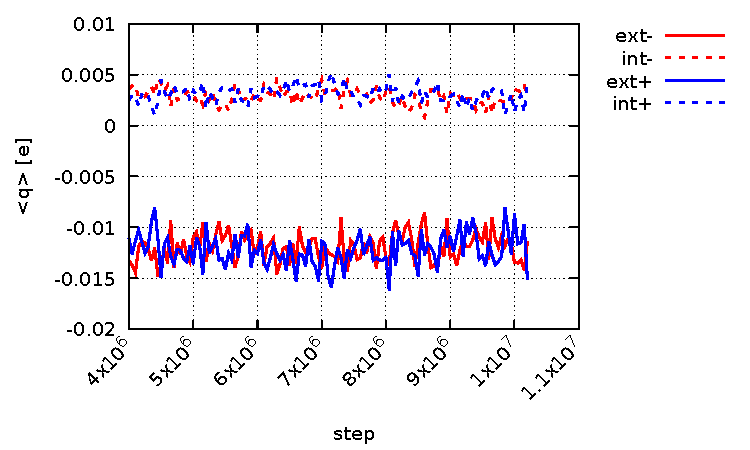
\includegraphics[width = \textwidth]{neutral_q-1.pdf}
        \caption{Pour le système non chargé}
        \label{fig:charges_groupes_neutral}
    \end{subfigure}
    
    \begin{subfigure}[t]{.49 \textwidth}
        \centering
        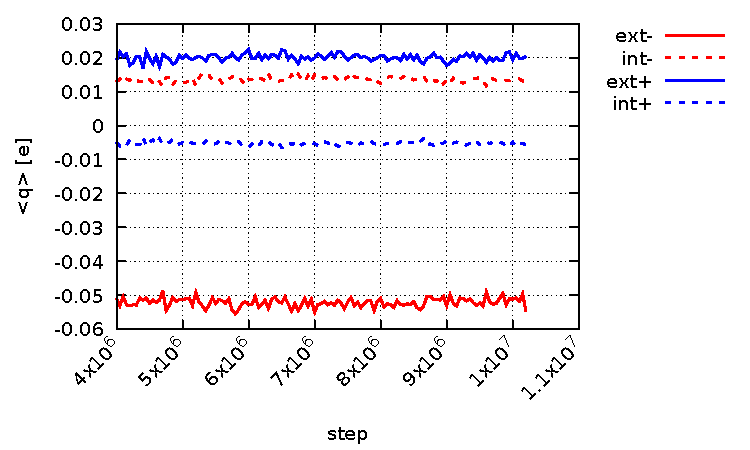
\includegraphics[width = \textwidth]{defected_q-1.pdf}
        \caption{Pour le système défectueux}
        \label{fig:charges_groupes_defected}
    \end{subfigure}

    \caption{Distribution des charges par groupes d'atomes. Les groupes d'atomes communs sont les carbones des couches intérieures et extérieures des deux électrodes ; Et pour le système défectueux il y a les atomes voisins du défaut}
    \label{fig:charges_groupes}
\end{figure}

\begin{figure}[h!]
    \centering
    \begin{subfigure}[t]{.49 \textwidth}
        \centering
        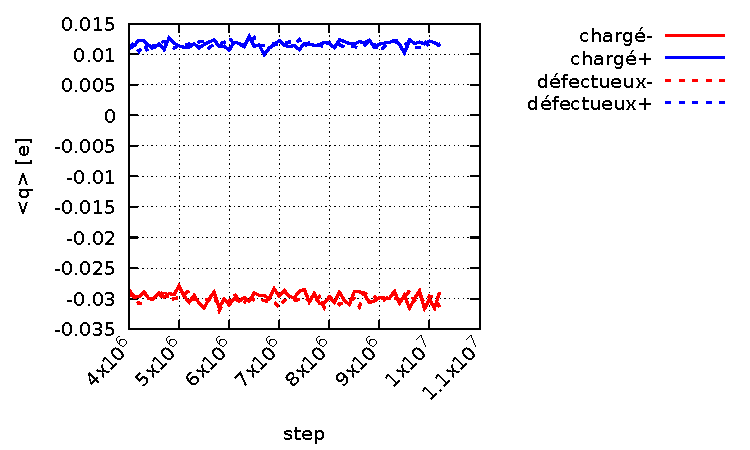
\includegraphics[width = \textwidth]{q_ch-sc-defected.pdf}
        \caption{Pour toutes les couches}
    \end{subfigure}%
    ~
    \begin{subfigure}[t]{.49 \textwidth}
        \centering
        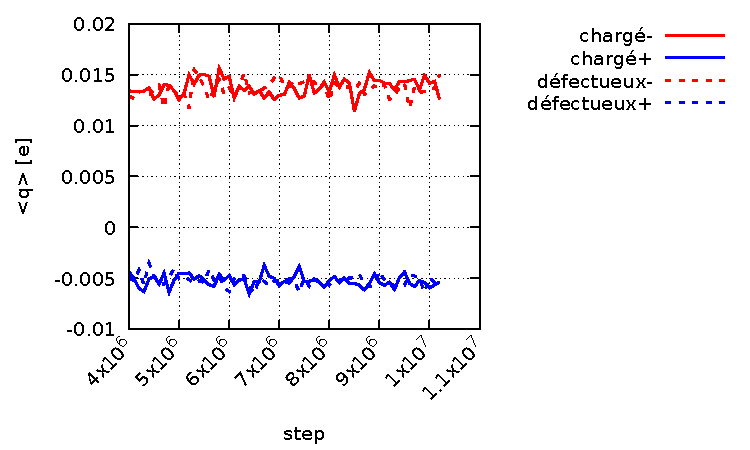
\includegraphics[width = \textwidth]{q_ch-sc-defected-inn.pdf}
        \caption{Pour les couches intérieures}
    \end{subfigure}

    \begin{subfigure}[t]{.49 \textwidth}
        \centering
        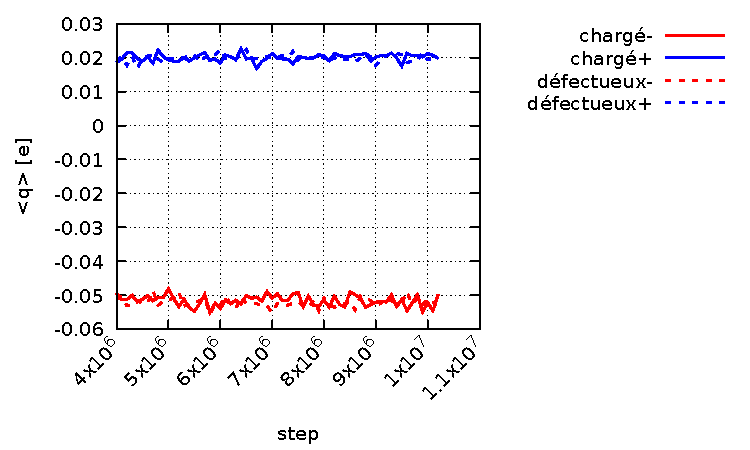
\includegraphics[width = \textwidth]{q_ch-sc-defected-out.pdf}
        \caption{Pour les couches extérieures}
    \end{subfigure}
    \caption{Comparaison des charges entre le système chargé et le système défectueux}
    \label{fig:comparaison_ch-sc-defected}
\end{figure}

\begin{figure}[h!]
    \centering
    \begin{subfigure}[t]{.49 \textwidth}
        \centering
        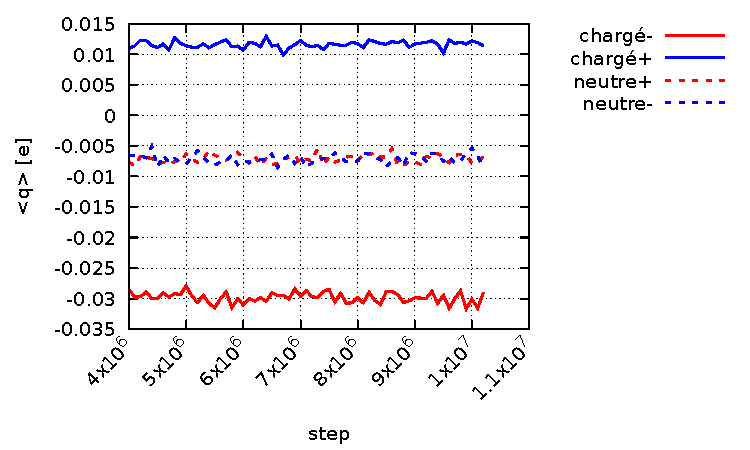
\includegraphics[width = \textwidth]{q_ch-sc-neutral.pdf}
        \caption{Pour toutes les couches}
    \end{subfigure}%
    ~
    \begin{subfigure}[t]{.49 \textwidth}
        \centering
        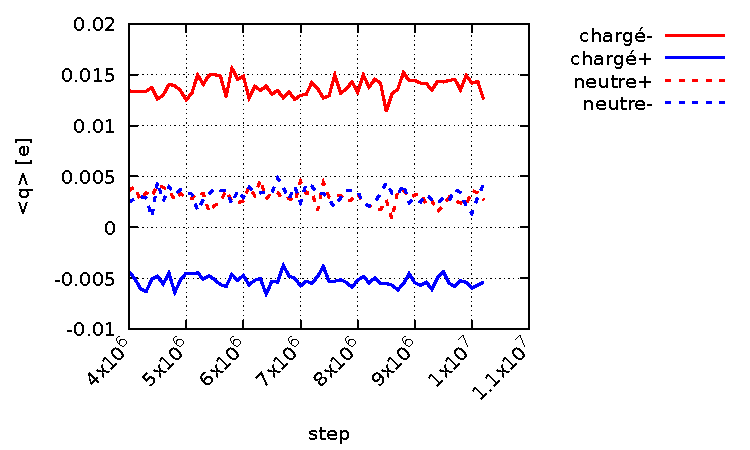
\includegraphics[width = \textwidth]{q_ch-sc-neutral-inn.pdf}
        \caption{Pour les couches intérieures}
    \end{subfigure}

    \begin{subfigure}[t]{.49 \textwidth}
        \centering
        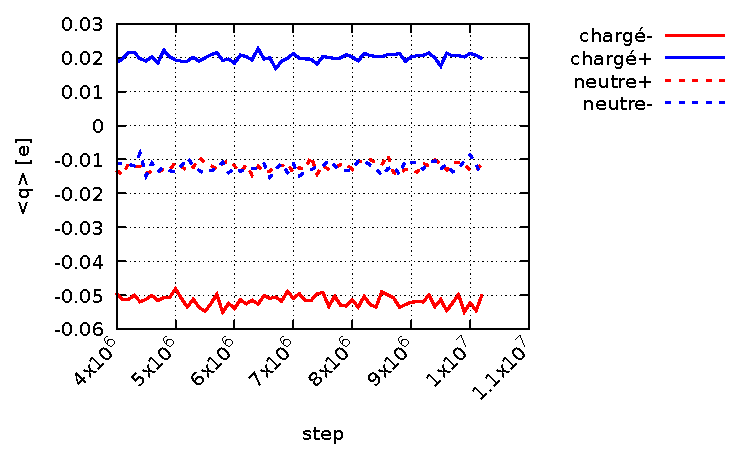
\includegraphics[width = \textwidth]{q_ch-sc-neutral-out.pdf}
        \caption{Pour les couches extérieures}
    \end{subfigure}
    \caption{Comparaison des charges entre le système chargé et le système non chargé}
    \label{fig:comparaison_ch-sc-neutral}
\end{figure}

\begin{table}[h!]
    \centering
    \begin{tabular}{c | c | c || c}
        \hline
        Système &Électrode &Couches &Moyenne des charges [\unit{\e}]\\
        \hline
        chargé &négative &toutes &\num{-0.0299}\\
         & &intérieures &\num{0.0138}\\
         & &extérieures &\num{-0.0517}\\
         &positive &toutes &\num{0.0116}\\
         & &intérieures &\num{-0.0052}\\
         & &extérieures &\num{0.0200}\\
        \hline
        neutre &négative &toutes &\num{-0.0070}\\
         & &intérieures &\num{0.0031}\\
         & &extérieures &\num{-0.0121}\\
        &positive &toutes &\num{-0.0071}\\
         & &intérieures &\num{0.0028}\\
         & &extérieures &\num{-0.0119}\\ 
        \hline
        défectueux &négative &toutes &\num{-0.0300}\\
         & &intérieures &\num{0.0135}\\
         & &extérieures &\num{-0.0519}\\
         &positive &toutes &\num{0.0116}\\
         & &intérieures &\num{-0.0052}\\
         & &extérieures &\num{0.0200}\\
        \hline
    \end{tabular}
    \caption{Tableau récapitulatif des moyennes des charges en fonction du groupe de carbone}
    \label{tab:comparaison_charges}
\end{table}

\clearpage

\textbf{Observations}\\
Pour les systèmes chargés (\autoref{fig:charges_groupes_ch-sc} et \ref{fig:charges_groupes_defected}, et \autoref{tab:comparaison_charges}), il semble que les charges des électrodes soient situées plutôt sur leurs couches extérieures : pour l'électrode négative les couches extérieures sont chargées négativement, tandis que pour l'électrode positive elles sont chargées positivement.

Pour le système neutre (\autoref{fig:charges_groupes_neutral}, et \autoref{tab:comparaison_charges}), nous pouvons voir un décalage de charges entre les couches : les couches extérieures sont chargées négativement tandis que les couches intérieures sont chargées positivement, de plus les couches extérieures sont plus chargées que les couches intérieures. Mais malgré ces décalages, les moyennes des charges sont quasimment les mêmes pour les deux électrodes et leurs couches respectives.

En comparant les systèmes chargés (\autoref{fig:comparaison_ch-sc-defected}, et \autoref{tab:comparaison_charges}), nous voyons que les charges des deux systèmes sont quasimment les mêmes pour les deux électrodes et leurs couches séparément.

En comparant les systèmes chargés au système non chargé (\autoref{fig:comparaison_ch-sc-neutral}, et \autoref{tab:comparaison_charges}), nous pouvons voir que pour les charges des électrodes des systèmes chargés sont presque à écarts égaux des charges du système non chargé. Cependant, l'écart de charges entre les couches intérieures et extérieures est plus grand pour l'électrode négative que pour l'électrode positive (\qtyrange[range-units = single]{125}{135}{\percent}).

\textbf{Interprétations}\\
La différence de charges entre les couches extérieures et intérieures peut avoir trois raisons :
\begin{itemize}
    \item La polarisation du système a pour conséquence d'attirer les charges d'une électrode vers l'autre ; Puisque le système est périodique selon la direction orthogonale aux surfaces des électrodes (selon la direction $[Oz)$), les charges d'une électrode sont attirées vers l'électrode opposée et son image périodique, c'est-à-dire vers les couches extérieures
    \item Au commencement de l'analyse des données (à partir de \qty{0.4}{\nano \second}), la double couche électrochimique (\edl{}) est déjà formée et les charges de chaque électrode sont concentrées à leurs interfaces avec l'électrolyte
    \item Les environnements des atomes de carbones influencent leurs propriétés (notamment leur charge) ; De plus, dans une approximation métallique les charges tendent à se diffuser vers la surface du métal
\end{itemize}

Quant au décalage de charges entre les couches du système non chargé, puisqu'il n'existe pas de différence de potentiel entre les électrodes il est possible que ce phénomène ne soit qu'une conséquence de l'interface entre l'électrode et l'électrolyte.

L'absence de différences notables entre les charges des systèmes chargés nous laisse penser que la présence du défaut n'influence pas la charge du système dans sa globalité.

Pour les écarts de charges entre les couches intérieures et extérieures du système chargé par rapport aux valeurs du système neutre, il n'y a pas de raison apparente. Cependant, le fait que pour les trois groupes d'atomes (couches intérieures, extérieures, et intégralité de l'électrode) il y ait un rapport d'environ $\num{1.25}\sim \num{1.35}$ nous laisse penser qu'il existe une raison sous-jacente et non évidente.

\clearpage
% Ions adsorption/displacement
    \subsubsection{Adsorption et déplacements des ions}

L'adsorption des ions est mesurée par deux grandeurs : la densité numérique d'ions dans l'électrolyte, et la fonction de ditribution radiale entre les ions et les carbones des électrodes.

Les \autoref{fig:densite} et \ref{fig:comparaison_densite} présentent la densité numérique d'ions dans l'électrolyte en fonction de la direction $[Oz)$ (correspondant à la direction orthogonale aux surfaces des électrodes) au début de l'analyse (à \qty{0.4}{\nano \second}) et à la fin (à \qty{1.0}{\nano \second}) pour les systèmes chargés et le système neutre.\\
Les \autoref{fig:rdf_ch-sc-neutral} et \ref{fig:rdf_ch-sc-defected}, elles montrent les \rdf{}s des ions sodium et hydroxyde de l'électrolyte par rapport aux carbones des couches extérieures des deux électrodes des trois systèmes. Et la \autoref{fig:rdf_sp} compare la \rdf{} des ions sodium et des carbones voisins du défaut du système défectueux à d'autres carbones.

\begin{figure}[h!]
    \centering
    \begin{subfigure}[t]{.49 \textwidth}
        \centering
        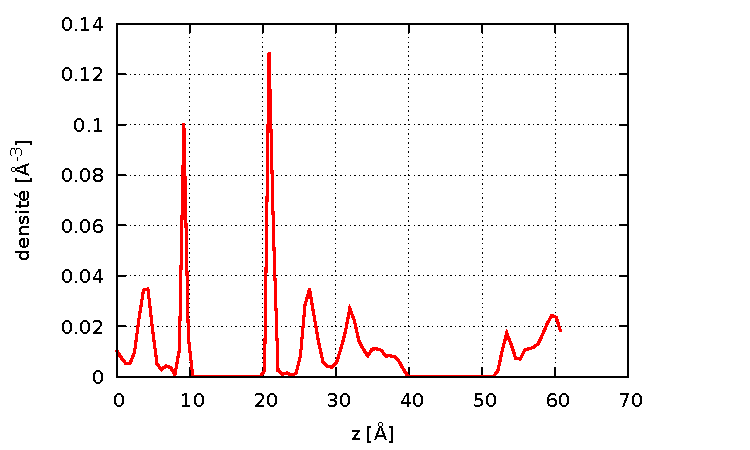
\includegraphics[width = \textwidth]{ch-sc_average_density.pdf}
        \caption{Pour le système chargé}
    \end{subfigure}%
    ~
    \begin{subfigure}[t]{.49 \textwidth}
        \centering
        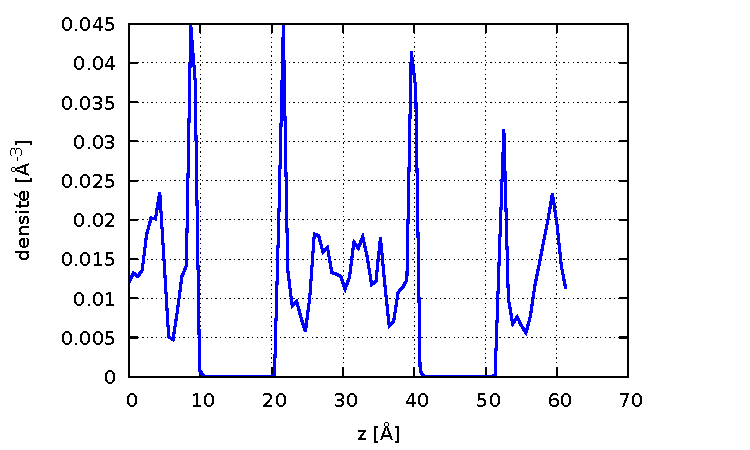
\includegraphics[width = \textwidth]{neutral_average_density.pdf}
        \caption{Pour le système non chargé}
    \end{subfigure}

    \begin{subfigure}[t]{.49 \textwidth}
        \centering
        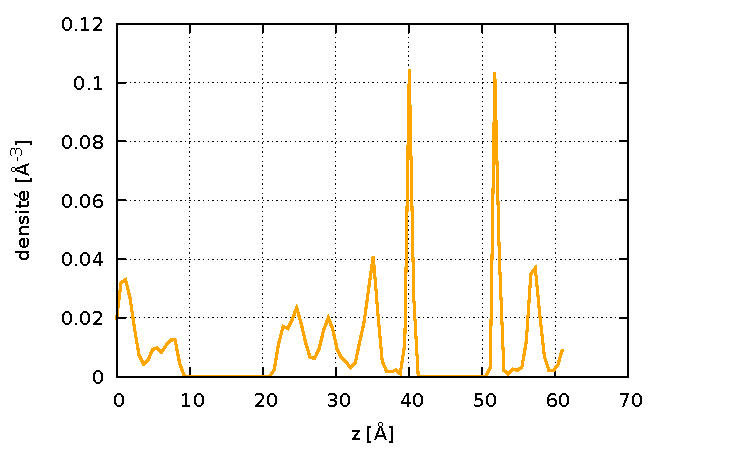
\includegraphics[width = \textwidth]{defected_average_density.pdf}
        \caption{Pour le système défectueux}
    \end{subfigure}
    \caption{Densités numériques moyennes d'ions sodium dans l'électrolyte}
    \label{fig:densite}
\end{figure}

\begin{figure}[h!]
    \centering
    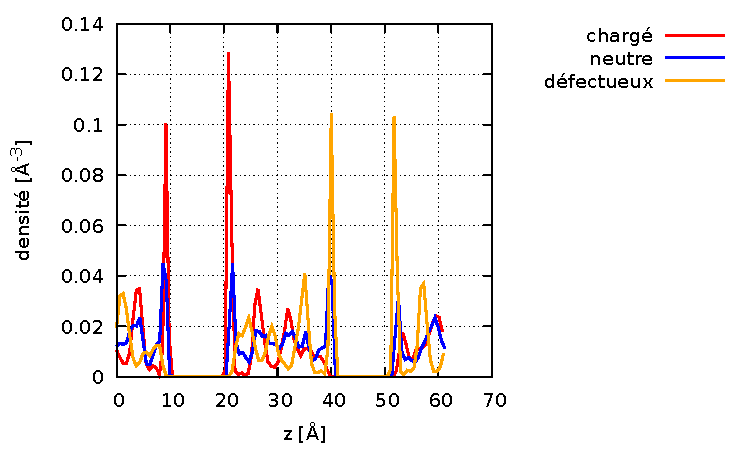
\includegraphics[width = \textwidth]{densities.pdf}
    \caption{Comparaisons des densités numériques moyennes. Le système défectueux a ses électrodes échangées (la positive à la place de la négative) par rapport au système chargé.}
    \label{fig:comparaison_densite}
\end{figure}

\begin{figure}[h!]
    \centering
    \begin{subfigure}[t]{.49 \textwidth}
        \centering
        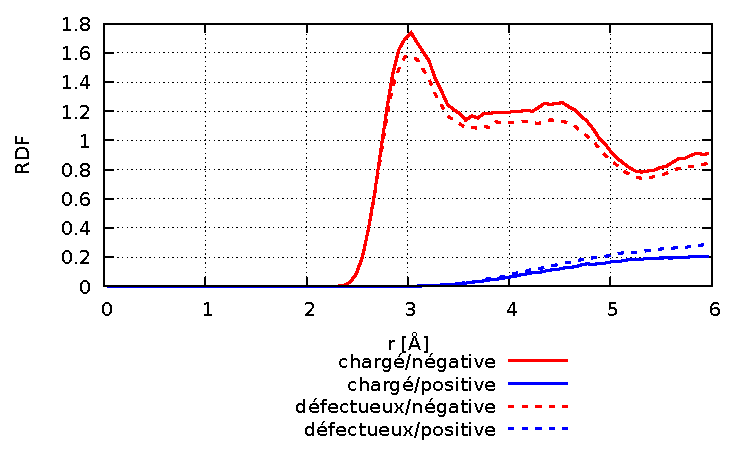
\includegraphics[width = \textwidth]{rdf_ch-sc-defected-Na.pdf}
        \caption{Pour les ions sodium}
    \end{subfigure}%
    ~
    \begin{subfigure}[t]{.49 \textwidth}
        \centering
        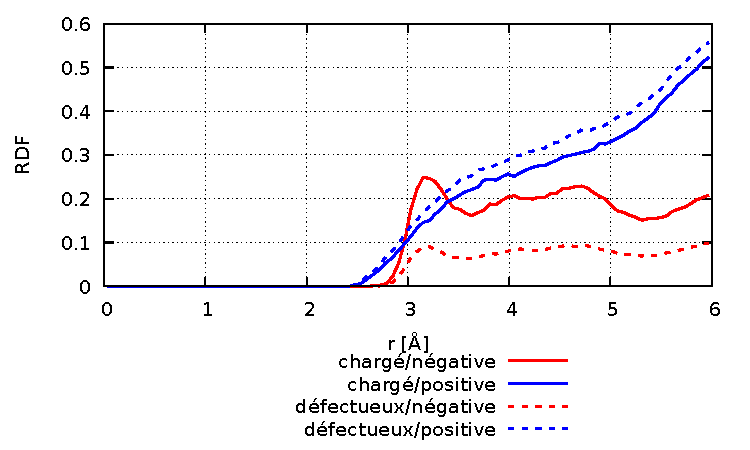
\includegraphics[width = \textwidth]{rdf_ch-sc-defected-OH.pdf}
        \caption{Pour les ions hydroxyde}
    \end{subfigure}

    \begin{subfigure}[t]{.49 \textwidth}
        \centering
        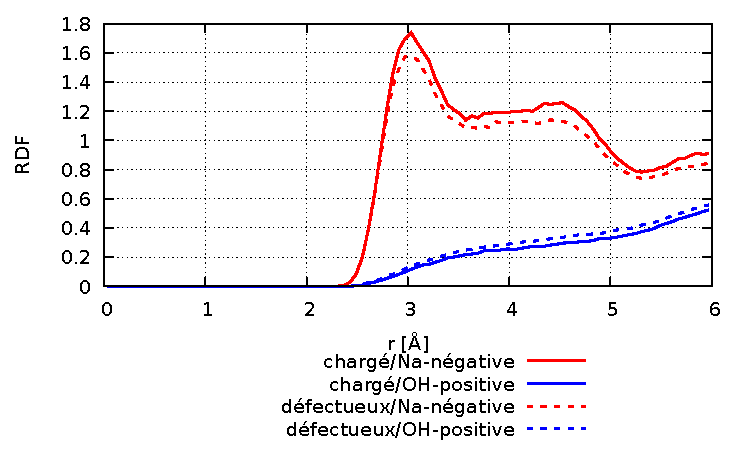
\includegraphics[width = \textwidth]{rdf_ch-sc-defected-NaOH.pdf}
        \caption{Pour tous les ions, par rapport à leurs électrodes respectives}
    \end{subfigure}
    \caption{Comparaison des \rdf{}s des ions par rapport aux carbones des électrodes entre le système chargé et le système défectueux}
    \label{fig:rdf_ch-sc-defected}
\end{figure}

\begin{figure}[h!]
    \centering
    \begin{subfigure}[t]{.49 \textwidth}
        \centering
        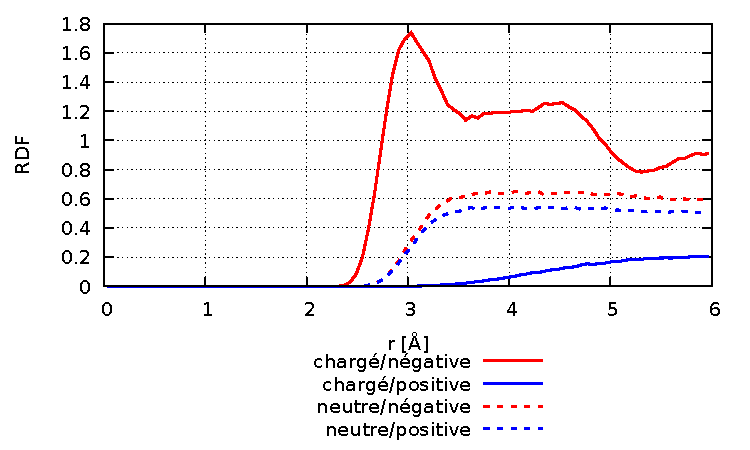
\includegraphics[width = \textwidth]{rdf_ch-sc-neutral-Na.pdf}
        \caption{Pour les ions sodium}
    \end{subfigure}%
    ~
    \begin{subfigure}[t]{.49 \textwidth}
        \centering
        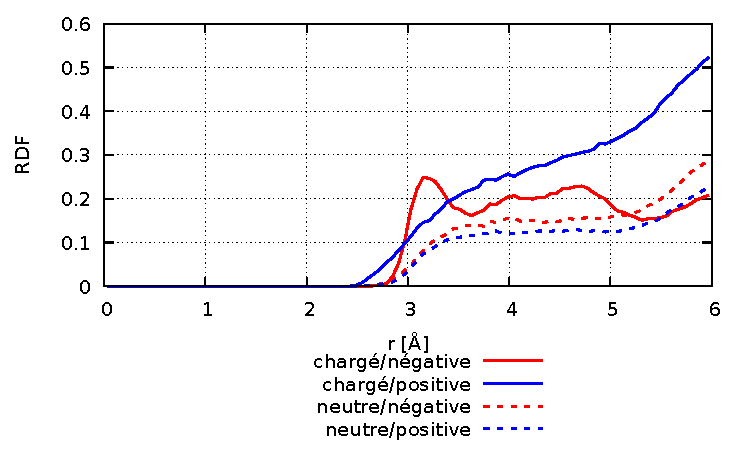
\includegraphics[width = \textwidth]{rdf_ch-sc-neutral-OH.pdf}
        \caption{Pour les ions hydroxyde}
    \end{subfigure}

    \begin{subfigure}[t]{.49 \textwidth}
        \centering
        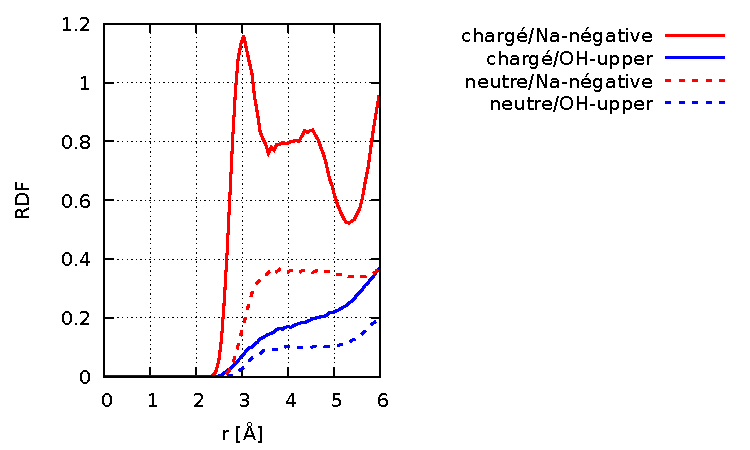
\includegraphics[width = \textwidth]{rdf_ch-sc-neutral-NaOH.pdf}
        \caption{Pour les tous ions, par rapport à leurs électrodes respectives}
    \end{subfigure}
    \caption{Comparaison des \rdf{}s des ions par rapport aux carbones des électrodes entre le système chargé et le système neutre}
    \label{fig:rdf_ch-sc-neutral}
\end{figure}

\begin{figure}[h!]
    \centering
    \begin{subfigure}[t]{.49 \textwidth}
        \centering
        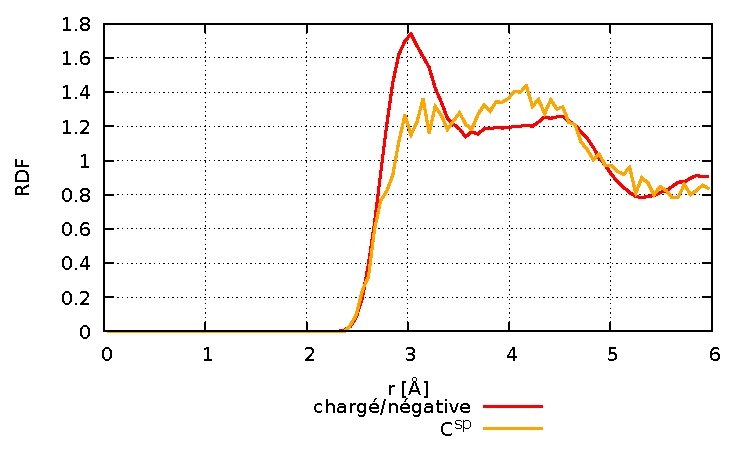
\includegraphics[width = \textwidth]{rdf_ch-sc-defected-sp.pdf}
        \caption{Avec les carbones de l'électrode négative du système chargé}
    \end{subfigure}%
    ~
    \begin{subfigure}[t]{.49 \textwidth}
        \centering
        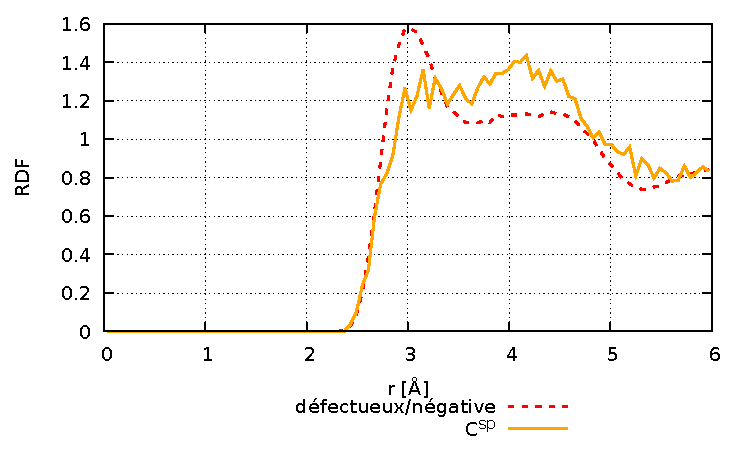
\includegraphics[width = \textwidth]{rdf_defected.pdf}
        \caption{Avec les carbones de l'électrode négative du système défectueux}
    \end{subfigure}
    \caption{Comparaison de la \rdf{} des ions sodium et des voisins du défaut}
    \label{fig:rdf_sp}
\end{figure}

\clearpage
\textbf{Observations}\\
Pour les densités numériques moyennes des ions sodium selon l'axe $[Oz)$ (\autoref{fig:densite}), nous pouvons dire que pour les systèmes chargés les ions sodium se regroupent près l'électrode négative (avec des pics de densité jusqu'à \num{4} fois plus grands qu'ailleurs dans l'électrolyte) ; Et pour le système neutre nous voyons des pics de densité moins important près des deux électrodes (environ \num{2} fois la valeur de la densité ailleurs dans l'électrolyte).

En observant attentivement, nous pouvons décerner un pattern pour les trois courbes : un pic intense près d'une des électrodes, puis une baisse de densité suivie de plusieurs pics à moyenne voire basse intensité.

En comparant les densités numériques des systèmes (\autoref{fig:comparaison_densite}), il est clair que les pics près des électrodes sont \num{2} à \num{3} fois plus intenses pour les systèmes chargés que pour le système non chargé.

En examinant les \rdf{}s, nous pouvons observer que :
\begin{itemize}
    \item la \rdf{} d'un ion est plus élevée et structurée lorsque prise par rapport aux carbones de l'électrode qui l'attire
    \item les \rdf{}s des systèmes chargés sont légèrement décalées mais dessinent les mêmes formes (\autoref{fig:rdf_ch-sc-defected})
    \item les \rdf{}s du système neutre sont plus uniformes que celles des systèmes chargés (\autoref{fig:rdf_ch-sc-neutral})
    \item pour tous les systèmes, les \rdf{}s des ions sodium sont globalement plus élevées et possèdent des pics plus prononcés que les \rdf{}s des ions hydroxyde
    \item la \rdf{} du sodium par rapport aux voisins du défaut est très similaire aux \rdf{}s par rapport aux autres carbones (\autoref{fig:rdf_sp})
\end{itemize}

\textbf{Interprétations}\\
Les différences de densités numériques entre les systèmes chargés et le système neutre semblent intuitives : les ions sodium sont plus dispersés pour le système neutre que pour le système chargé, à cause de l'application de la différene de potentiel, et les pics de densité près de l'électrode négative sont plus importants pour les sytèmes chargés à cause de la différence de potentiel appliquée.

Puisque les densités numériques des trois systèmes montrent un même pattern, il est très probable que ce ne soit pas un hasard : nous pouvons penser qu'une couche d'ions est fortement attirée par l'électrode, et le reste des ions en excès reste dans une couche plus éloignée, dite de \emph{diffusion}.

À cause de leur charge négative, même en l'absence de polarisation (\autoref{tab:comparaison_charges}), les deux électrodes du système neutre attirent les ions sodium de l'électrolyte.

Les \rdf{}s nous permettent d'étayer ces réflexions :
\begin{itemize}
    \item puisque les ions sont attirés par leur électrode opposée, la \rdf{} correspondante sera plus intense. Avec le pattern de densité décrit précédemment, il est également normal d'observer des pics pour les \rdf{}s
    \item à l'inverse pour le système non chargé, les \rdf{}s seront plus uniformes et moins intenses
\end{itemize}

Malgré cela, la différence des \rdf{}s des ions hydroxyde par rapport aux ions sodium n'est pas simple à interpréter : elle peut venir d'un problème d'implémentation ou d'un phénomène physique.\\
En effet, puisque le potentiel que nous utilisons est réactif, les atomes n'appartiennent pas à des molécules prédéfinies et ils peuvent alors se lier et se séparer les uns des autres. Cela rend alors le travail de sélection des ions plus difficile. Pour cette étude, nous avons choisi de faire simplement : à chaque image de la trajectoire de simulation, nous avons sélectionné tous les atomes d'oxygène et d'hydrogène, calculé les liaisons pouvant exister entre eux, et sélectionné seulement les atomes d'oxygène possédant moins de deux liaisons. Malgré qu'une bonne partie devrait être de \emph{vrais} ions hydroxyde, les atomes sélectionnés sont plus nombreux que le nombre initial d'ions de l'électrolyte pouvant ainsi causer des erreurs de calculs.\\
S'il n'y avait pas d'erreur, alors il est probable que cette différence soit causée par les réactions entre les ions hydroxyde et les molécules d'eau, perturbant la distribution des ions autour des électrodes.\\
Dans tous les cas, nous ne pouvons pas affirmer si les \rdf{}s des ions hydroxydes sont différentes de celles des ions sodium à cause de la charge différente des électrode (\autoref{tab:comparaison_charges}) ou à cause de la nature des ions.

Enfin, la comparaison des \rdf{}s du sodium par rapport aux voisins du défaut et des carbones des électrodes négatives des systèmes chargés ne montre pas de grande différence. Cela pourrait vouloir dire qu'un tel défaut ou un défaut seul ne permette pas de voir une grande différence ; Cette différence pourrait surgir avec un système de plus grande taille, ou pour des simulations plus longues avec de plus grandes statistiques.

% Discussion of the study
    \subsection{Discussion}

Les résultats obtenus pourraient être améliorés pour une prochaine étude en :
\begin{itemize}
    \item équilibrant la simulation principale \emph{avant} d'appliquer la différence de potentiel afin de pouvoir observer sur un même système la formation de l'\edl{}, les variations de charges des électrodes (lorsque le voltage se met en place), et pouvoir calculer deux densités numériques moyennes d'ions différentes [avant et après la mise en place de la différence de potentiel]
    \item augmentant la taille du système, de manière à obtenir plus de statistiques
    \item complexifiant progressivement le système, par exemple en créant un pore artificiel dans l'électrode, ou encore en créant un tunnel dans l'électrode pour simuler un réseau de pore, dans le but de voir l'influence d'une telle modification sur le système
    \item remplaçant les ions hydroxydes initiaux par d'autres anions, comme par exemple les ions chlore, afin de les tracer plus facilement dans l'électrolyte et de déterminer si les différences que nous avons observé provenaient de la nature des ions utilisés ou du système lui-même
\end{itemize}
